\documentclass[12pt, a4paper]{article}
\usepackage{../../../myconfig} % Gọi file cấu hình từ ngoài gốc vào

% ==========================================
% BẮT ĐẦU NỘI DUNG TÀI LIỆU
% ==========================================
\begin{document}

% Truyền 3 tham số: {Nhãn cam} {Chữ to chính giữa} {Chữ ở góc phải Header}
\titlebox{Chủ đề: Hàm số}{BT điểm danh hàm số bậc 3}{Hàm số: Hàm bậc 3}

\questionLinesManual{3}{1}{Đồ thị của hàm số dưới đây có dạng như đường cong bên?

\begin{center}
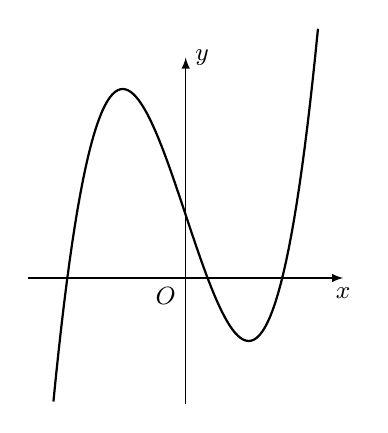
\begin{tikzpicture}[>=latex, scale=0.8]
    % Hệ trục tọa độ
    \draw[->] (-2.5,0) -- (2.5,0) node[below] {\small $x$};
    \draw[->] (0,-2) -- (0,3.5) node[right] {\small $y$};
    \node[below left] at (0,0) {\small $O$};
    
    % Đồ thị hàm bậc 3: y = -x^3 + 3x + 1
    \draw[thick, samples=100, domain=-2.1:2.1] 
        plot (\x, {\x*\x*\x - 3*\x + 1});
\end{tikzpicture}
\end{center}

}{
    \begin{tasks}(4)
        \task \( y = x^3 - 3x + 1 \)
        \task \( y = x^4 - 2x^2 + 1 \)
        \task \( y = -x^4 + 2x^2 + 1 \)
        \task \( y = -x^3 + 3x + 1 \)
    \end{tasks}
}

\questionLinesManual{5}{2}{Đồ thị hàm số nào sau đây có dạng như hình vẽ?

\begin{center}
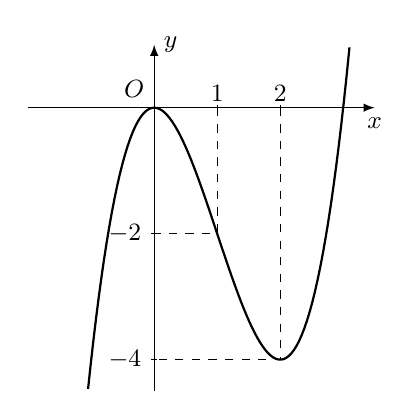
\begin{tikzpicture}[>=latex, scale=0.8]
    % Hệ trục tọa độ
    \draw[->] (-2,0) -- (3.5,0) node[below] {\small $x$};
    \draw[->] (0,-4.5) -- (0,1) node[right] {\small $y$};
    \node[above left] at (0,0) {\small $O$};
    
    % Đánh dấu các mốc
    \foreach \x in {1,2} {
         \draw (\x,0.05) -- (\x,-0.05)  node[above] {\small $\x$};
    }
    \foreach \y in {-4,-2} {
          \draw (0.05,\y) -- (-0.05,\y)   node[left] {\small $\y$};
    }
    
    % Đồ thị hàm bậc 3: y = -x^3 + 3x
    \draw[thick, samples=100, domain=-1.05:3.1] 
        plot (\x, {\x*\x*\x - 3*\x*\x});
    
    % Đánh dấu điểm cực trị
    \draw[dashed] (1,0) -- (1,-2) -- (0,-2);
    \draw[dashed] (2,0) -- (2,-4) -- (0,-4);
\end{tikzpicture}

\end{center}

}{
    \begin{tasks}(4)
        \task \( y = x^3 - 3x^2 \)
        \task \( y = x^3 + 3x \)
        \task \( y = -x^3 + 3x^2 \)
        \task \( y = -x^3 + 3x \)
    \end{tasks}
}

\questionLinesManual{3}{3}{Hình vẽ sau là bảng biến thiên của hàm số nào dưới đây?

\begin{center}

\begin{tikzpicture}
    \tkzTabInit[lgt=1.5, espcl=2.5]
    {$x$ /1, $y'$ /1, $y$ /2.5}
    {$-\infty$, $-1$, $1$, $+\infty$}
    \tkzTabLine{, -, 0, +, 0, -, }
    \tkzTabVar{+/ $+\infty$ / , -/ $-5$ / , +/ $3$ / , -/ $-\infty$ /}
\end{tikzpicture}
\end{center}

}{
    \begin{tasks}(4)
        \task \( y = -2x^4 + x^2 - 1 \)
        \task \( y = \dfrac{-2x + 7}{x + 3} \)
        \task \( y = -2x^2 + x - 1 \)
        \task \( y = -2x^3 + 6x - 1 \)
    \end{tasks}
}

\questionLinesManual{3}{4}{Cho hàm số \( y = f(x) = ax^3 + bx^2 + cx + d \) (\( a \neq 0 \)) có đồ thị như hình vẽ.

\begin{center}
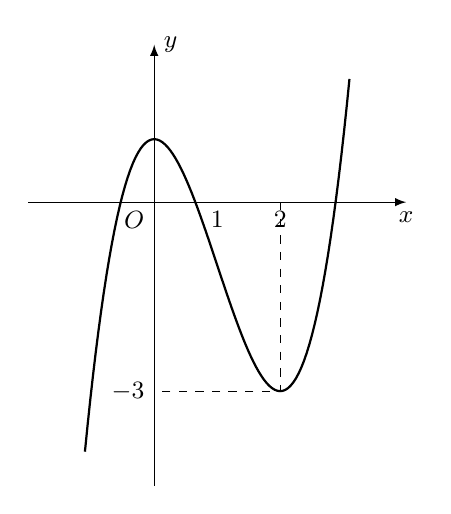
\begin{tikzpicture}[>=latex, scale=0.8]
    % Hệ trục tọa độ
    \draw[->] (-2,0) -- (4,0) node[below] {\small $x$};
    \draw[->] (0,-4.5) -- (0,2.5) node[right] {\small $y$};
    \node[below left] at (0,0) {\small $O$};
    
    
    % Đồ thị hàm bậc 3: y = x^3 - 3x
    \draw[thick, samples=100, domain=-1.1:3.1] 
        plot (\x, {\x*\x*\x - 3*\x*\x + 1});
    
    % Đánh dấu điểm cực trị
    \draw[dashed] (2,0) -- (2,-3) -- (0,-3);
    \node[below] at (1,0) {\small $1$};
    \node[below] at (2,0) {\small $2$};
    \node[left] at (0,-3) {\small $-3$};
\end{tikzpicture}
\end{center}

Số nghiệm của phương trình \( f(x) = -2 \) là}{
    \begin{tasks}(4)
        \task $2$
        \task $0$
        \task $1$
        \task $3$
    \end{tasks}
}

\questionLinesManual{5}{5}{Cho hàm số \( y = ax^3 + bx^2 + cx + d \) có đồ thị như hình vẽ. Khẳng định nào dưới đây đúng?

\begin{center}
\begin{tikzpicture}[>=latex, scale=0.8]
    % Hệ trục tọa độ
    \draw[->] (-3.5,0) -- (4,0) node[below] {\small $x$};
    \draw[->] (0,-4.5) -- (0,2) node[right] {\small $y$};
    \node[below left] at (0,0) {\small $O$};   
    % Đồ thị hàm bậc 3: y = x^3 - 3x
    \draw[thick, samples=100, domain=-2:2] 
        plot (\x, {-\x*\x*\x + 3*\x-1});
   
\end{tikzpicture}
\end{center}

}{
    \begin{tasks}(2)
        \task Hàm số đã cho đồng biến trên khoảng \((-\infty; +\infty)\).
        \task \( a > 0, d < 0 \).
        \task \( a < 0, d > 0 \).
        \task Hàm số đã cho có hai điểm cực trị.
    \end{tasks}
}

\questionLinesManual{5}{6}{Cho đường cong \( (C) : y = ax^3 + bx^2 + cx + d \) có đồ thị như hình bên.

\begin{center}
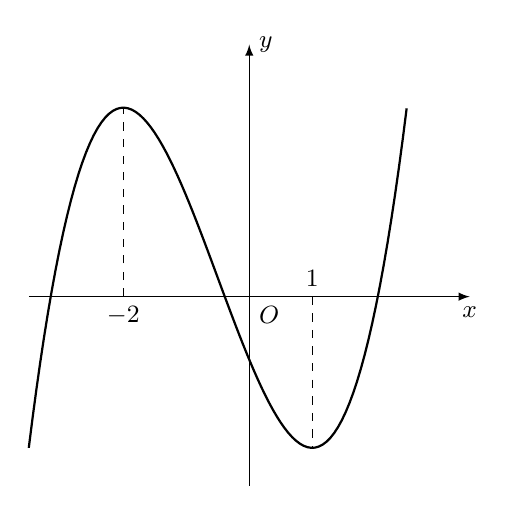
\begin{tikzpicture}[>=latex, scale=0.8]
    % Hệ trục tọa độ
    \draw[->] (-3.5,0) -- (3.5,0) node[below] {\small $x$};
    \draw[->] (0,-3) -- (0,4) node[right] {\small $y$};
    \node[below right] at (0,0) {\small $O$};
   
    % Đồ thị hàm bậc 3: y = -x^3 + 3x^2 + 2
    \draw[thick, samples=100, domain=-3.5:2.5] 
        plot (\x, {0.2*(2*\x*\x*\x + 3*\x*\x - 12*\x)-1});
    \draw[dashed] (1,0) -- (1,-2.4);
    \draw[dashed] (-2,0) -- (-2,3);
    \node[above] at (1,0) {\small $1$};
    \node[below] at (-2,0) {\small $-2$};
\end{tikzpicture}
\end{center}

Khẳng định nào sau đây là đúng?}{
    \begin{tasks}(2)
        \task \( a > 0, b < 0, c < 0, d < 0 \)
        \task \( a > 0, b > 0, c < 0, d > 0 \)
        \task \( a < 0, b > 0, c > 0, d < 0 \)
        \task \( a > 0, b > 0, c < 0, d < 0 \)
    \end{tasks}
}

\questionLinesManual{5}{7}{Hàm số \( y = ax^3 + bx^2 + cx + d \) có đồ thị như hình vẽ bên dưới:

\begin{center}

\begin{tikzpicture}[>=latex, scale=0.8]
    % Hệ trục tọa độ
    \draw[->] (-2,0) -- (6,0) node[below] {\small $x$};
    \draw[->] (0,-4) -- (0,4) node[right] {\small $y$};
    \node[below right] at (0,0) {\small $O$};
    
   
    % Đồ thị hàm bậc 3: y = x^3 - 3x
    \draw[thick, samples=100, domain=-1.5:5.1] 
        plot (\x, {-0.25*(\x+1)*(\x-3)*(\x-4)});
  
\end{tikzpicture}
\end{center}

Khẳng định nào là đúng?}{
    \begin{tasks}(2)
        \task \( a < 0, b < 0, c < 0, d < 0 \)
        \task \( a > 0, b > 0, c > 0, d < 0 \)
        \task \( a < 0, b > 0, c < 0, d < 0 \)
        \task \( a > 0, b < 0, c > 0, d > 0 \)
    \end{tasks}
}


\questionLinesManual{5}{8}{Cho hàm số \( f(x) = ax^3 + bx^2 + cx + d \) (\( a, b, c, d \in \mathbb{R} \)) có bảng biến thiên như sau:

\begin{center}

\begin{tikzpicture}
    \tkzTabInit[lgt=1.5, espcl=2.5]
    {$x$ /1, $f'(x)$ /1, $f(x)$ /2.5}
    {$-\infty$, $-2$, $0$, $+\infty$}
    \tkzTabLine{, +, 0, -, 0, +, }
    \tkzTabVar{-/ $-\infty$ / , +/ $1$ / , -/ $-1$ / , +/ $+\infty$ /}
\end{tikzpicture}
\end{center}

Có bao nhiêu số dương trong các số \( a, b, c, d \)?}{
    \begin{tasks}(4)
        \task $3$
        \task $4$
        \task $2$
        \task $1$
    \end{tasks}
}

\questionLinesManual{8}{9}{Tìm điểm \( M \) có hoành độ âm trên đồ thị \( (C) \): \( y = \dfrac{1}{3}x^3 - x + \dfrac{2}{3} \) sao cho tiếp tuyến tại \( M \) vuông góc với đường thẳng \( y = -\dfrac{1}{3}x + \dfrac{2}{3} \).}{
    \begin{tasks}(4)
        \task \( M\left(-1; \dfrac{4}{3}\right) \)
        \task \( M(-2; 0) \)
        \task \( M\left(2; \dfrac{4}{3}\right) \)
        \task \( M(-2; -4) \)
    \end{tasks}
}

\questionLinesManual{5}{10}{Số giao điểm của đồ thị hàm số \( y = x^3 - 5x^2 \) và đồ thị hàm số \( y = -x^2 + 3x \) là}{
    \begin{tasks}(4)
        \task $3$
        \task $1$
        \task $2$
        \task $0$
    \end{tasks}
}
\end{document}
